\documentclass{article}
\usepackage{graphicx}

\title{CSCI-7000 — Infectious Disease Modeling Final Project}
\author{Sahana Balaji and Brenna Neeland}
\date{April 29, 2024}

\begin{document}

\maketitle

\section{Immunosenescence and its Function in Mathematical Modeling of Infectious Disease and Vaccination Modeling}
\textbf{Sahana Balaji and Brenna Neeland}\\
\texttt{Sahana.Balaji@Colorado.edu \& Brenna.Neeland@Colorado.edu}

\section{Introduction}
Varying factors can contribute to susceptibility to disease among populations. One particular factor to consider is age and the development of immunosenescence. Immunosenescence is the alteration of immune function, typically thymic involution causing the decreased functions of T and B cells, due to aging \cite{rink2022}. [Expand on processes metabolically] << more lit review. Both of these cell types are involved in the acquisition or antigen-specific immune response such that they are the only cells in an organism that can recognize and respond to that specific antigen epitope \cite{cano2013}. In immunosenescence, the number of memory T and B cells increase, while the response to new antigens decreases. Similarly, this decreases the function of granulocytes, macrophages, and NK cells \cite{rink2022}. 

\subsection{Thesis}
The importance of immunosenescence and aging was especially emphasized during the COVID-19 pandemic in 2020. Increased susceptibility to disease due to immunosenescence could play a huge role in the way mathematical and computational methods model disease and immunity as provided by vaccinations. This project seeks to explore how immunosenescence can be mathematically modeled using an SEIRS model, and how this idea can be applied to vaccination models. 

\section{Method}
In order to analyze varying susceptibility among different age groups, an SEIRS model was formed and modified to include variable T. T represents varying loss of immunity due to immunosenescence. This allowed us to form a set of ordinary differential equations (ODEs) with a varied T based on age. Furthermore, a contact matrix was formed for the varying age groups using a total population size of 145 (55 parents, 30 children, and 60 grandparents). We then generated code to compute these varying $R_0$ values. We then saved these results to a CSV file (\texttt{simulation\_results.csv}). We then manipulated this data under the influence of a Leaky Vaccination Model with varying Vaccine Efficacy (VE). We analyzed when VE was 0, 1, and 0.8. Each age group was visualized using bar charts generated with the Matplotlib library in Python.

\section{Results}
% JPEGs
\begin{figure}[htbp]
    \centering
    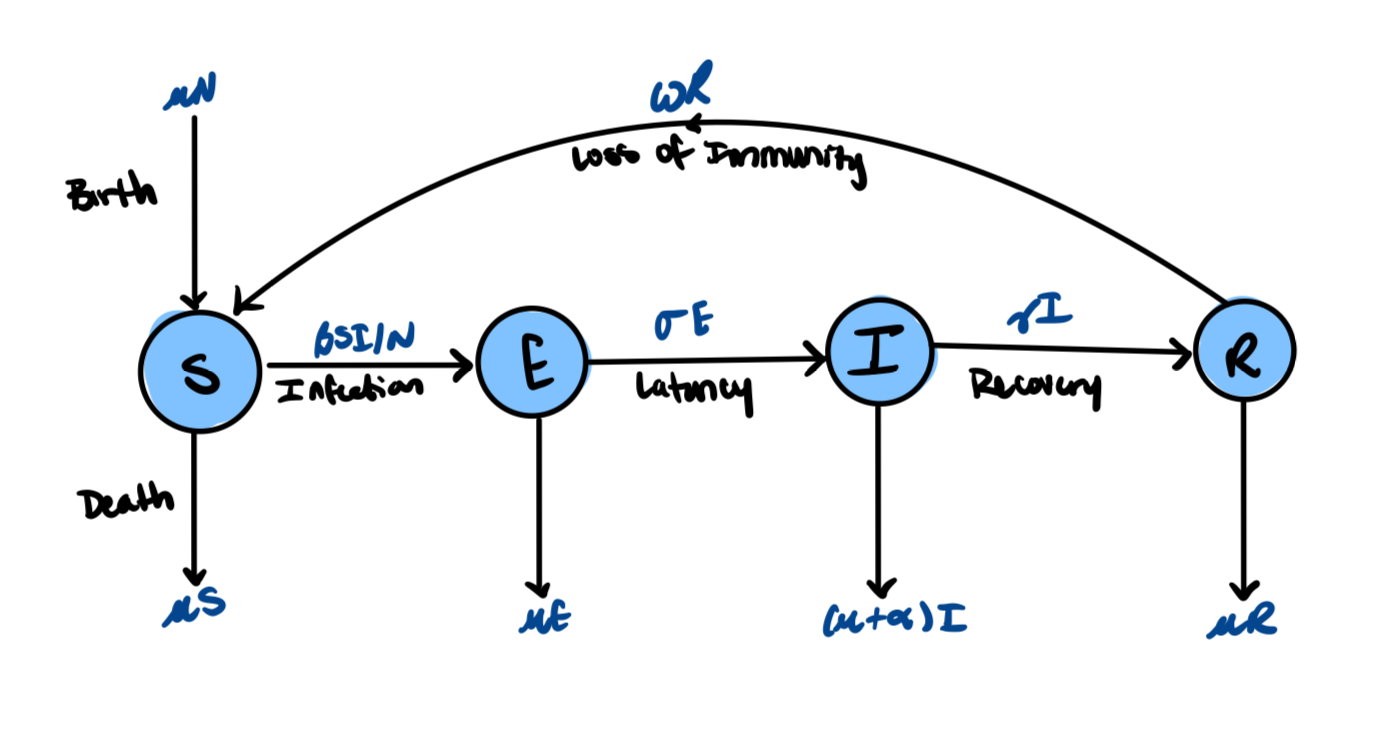
\includegraphics[width=0.8\textwidth]{seirs.jpeg}
    \caption{SEIRS Model}
    \label{fig:SEIRS}
\end{figure}

\begin{figure}[htbp]
    \centering
    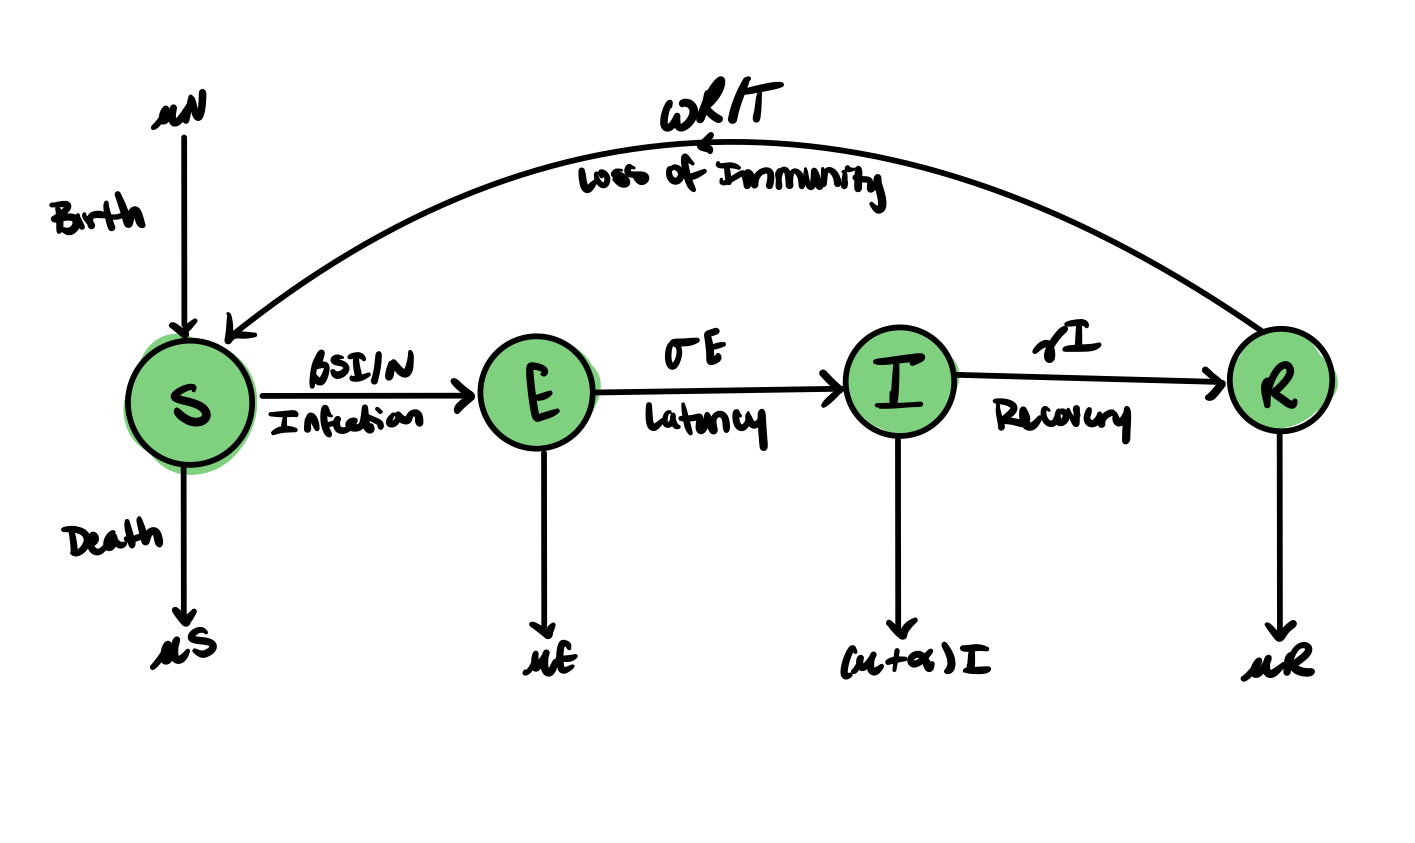
\includegraphics[width=0.8\textwidth]{seirsM.jpeg}
    \caption{Modified SEIRS Model}
    \label{fig:Immunosenscence Model}
\end{figure}

%PNGs
\begin{figure}[htbp]
    \centering
    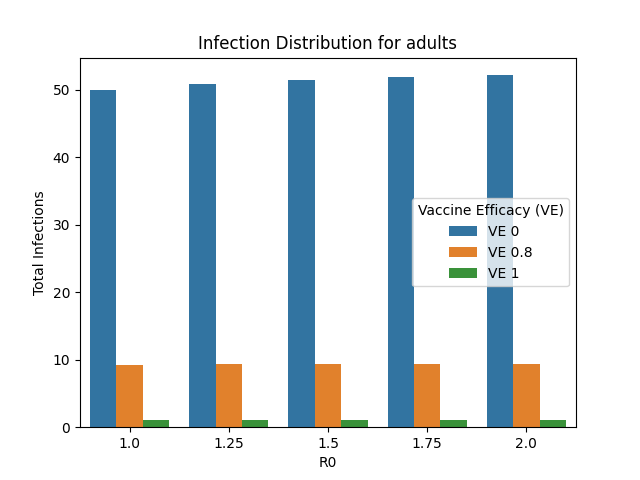
\includegraphics[width=0.8\textwidth]{adults}
    \caption{Adults Histogram}
    \label{fig:adults} % Add label for referencing
\end{figure}

As shown in Figure \ref{fig:adults}, ...

\begin{figure}[htbp]
    \centering
    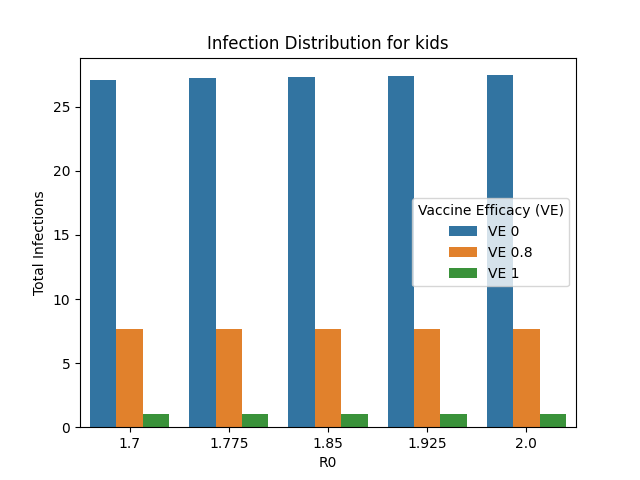
\includegraphics[width=0.8\textwidth]{kids}
    \caption{Kids Histogram}
    \label{fig:kids} 
\end{figure}

As shown in Figure \ref{fig:kids}, ...

\begin{figure}[htbp]
    \centering
    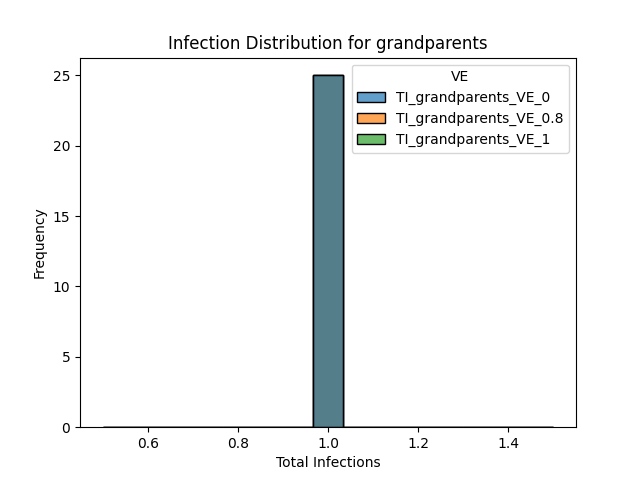
\includegraphics[width=0.8\textwidth]{grandparents}
    \caption{Grandparents Histogram}
    \label{fig:grandparents} 
\end{figure}

As shown in Figure \ref{fig:grandparents}, ...

\section{Conclusion}

\section{Discussion}

\section*{References}

\begin{enumerate}
    \item Bjørnstad, O.N., Shea, K., Krzywinski, M. et al. The SEIRS model for infectious disease dynamics. Nat Methods 17, 557–558 (2020). \texttt{https://doi.org/10.1038/s41592-020-0856-2}
    
    \item Chapter 5: Introduction to T and B lymphocytes. (Book citation)
    
    \item Liu, Z., Liang, Q., Ren, Y. et al. Immunosenescence: molecular mechanisms and diseases. Sig Transduct Target Ther 8, 200 (2023). \texttt{https://doi.org/10.1038/s41392-023-01451-2}
    
    \item Rink, L., Wessels, I. (2022). Immunosenescence. In N. Rezaei (Ed.), Encyclopedia of Infection and Immunity (pp. 259-276). Elsevier. \texttt{https://doi.org/10.1016/B978-0-12-818731-9.00072-0}
    
    \item Mittelbrunn, M., Kroemer, G. Hallmarks of T cell aging. Nat Immunol 22, 687–698 (2021). \texttt{https://doi.org/10.1038/s41590-021-00927-z}
    
    \item Yousefzadeh, M.J., Flores, R.R., Zhu, Y. et al. An aged immune system drives senescence and ageing of solid organs. Nature 594, 100–105 (2021). \texttt{https://doi.org/10.1038/s41586-021-03547-7}
\end{enumerate}

\end{document}
